\documentclass[onecolumn,a4paper,10pt]{article}
\usepackage{graphicx}
\usepackage{amsmath}

\begin{document}

\title{Lecture 8 - Error function}
\author{Jonas Hjorth Knudsen\\ 201406333}
\date{\today}

\maketitle

\section{Error function}

The errorfunction is defined as equation~\eqref{eq:errFun} and an example is plotted in Figure~\ref{fig:errFun} from $x = -3$ to $x = 3$ in steps of $0.05$ with the use of the programming language C.

\begin{align}
	\operatorname{erf}(x) &= \frac{1}{\sqrt{\pi}} \int_{-x}^{x} \! e^{-t^2} \, \mathrm{d}t \nonumber \\
	       &= \frac{2}{\sqrt{\pi}} \int_0^{x} \! e^{-t^2} \, \mathrm{d}t \label{eq:errFun}
\end{align}


\begin{figure}[!htbp]
	\centering
	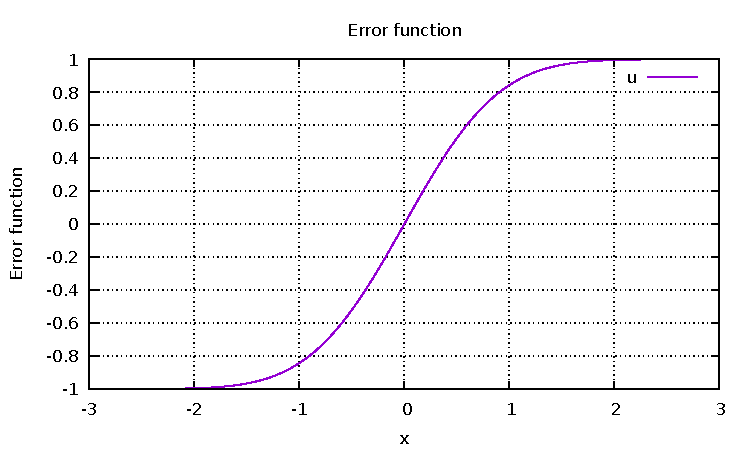
\includegraphics{plotErrorFun.pdf}
	\caption{Error function plotted from $x = -3$ to $x = 3$ in steps of $0.05$ by using equation~\eqref{eq:errFun} in the programming language C.}
	\label{fig:errFun}
\end{figure}


\end{document}
